\documentclass[english]{article}
\usepackage[LGR,T1]{fontenc}
\usepackage[latin9]{inputenc}
\pagestyle{headings}
\usepackage{color}
\usepackage[british,UKenglish]{babel}
\usepackage{float}
\usepackage{calc}
\usepackage{textcomp}
\usepackage{url}
\usepackage{amsmath}
\usepackage{amsthm}
\usepackage{amssymb}
\usepackage{graphicx}
\usepackage{esint}
\usepackage[unicode=true]
 {hyperref}


\usepackage{bera}

\makeatletter

%%%%%%%%%%%%%%%%%%%%%%%%%%%%%% LyX specific LaTeX commands.
\DeclareRobustCommand{\greektext}{%
  \fontencoding{LGR}\selectfont\def\encodingdefault{LGR}}
\DeclareRobustCommand{\textgreek}[1]{\leavevmode{\greektext #1}}
\ProvideTextCommand{\~}{LGR}[1]{\char126#1}

%% Because html converters don't know tabularnewline
\providecommand{\tabularnewline}{\\}
%% A simple dot to overcome graphicx limitations
\newcommand{\lyxdot}{.}


%%%%%%%%%%%%%%%%%%%%%%%%%%%%%% Textclass specific LaTeX commands.
\numberwithin{equation}{section}
\numberwithin{figure}{section}

%%%%%%%%%%%%%%%%%%%%%%%%%%%%%% User specified LaTeX commands.
\usepackage{stmaryrd}
\definecolor{colKeys}{rgb}{0,0,1}
\definecolor{colIdentifier}{rgb}{0,0,0}
\definecolor{colComments}{rgb}{0.53, 0.66, 0.42}
\definecolor{colString}{rgb}{0.87, 0.36, 0.51}
\definecolor{barColor}{rgb}{0.43, 0.5, 0.5}
% Added by lyx2lyx
\renewcommand{\textendash}{--}
\renewcommand{\textemdash}{---}

\makeatother

\usepackage{listings}
\lstset{language=Matlab,
float=hbp,
basicstyle={\footnotesize\ttfamily},
identifierstyle={\color{colIdentifier}},
keywordstyle={\color{colKeys}},
stringstyle={\color{colString}},
commentstyle={\itshape\color{colComments}},
columns=fixed,
tabsize=2,
extendedchars=true,
showspaces=false,
showstringspaces=false,
captionpos=t,
backgroundcolor={\color{white}},
framexleftmargin=1pt,
frame=l}
\renewcommand{\lstlistingname}{Listing}
\title{PsPM Release Notes\\ ~\\ Version 6.1.2}

\begin{document}
\maketitle
\date
\pagebreak


\tableofcontents{}
\pagebreak

\section{PsPM Version 3.0}

\subsection*{Import}

\subsubsection*{New data types were implemented}
\begin{itemize}
\item Noldus Observer compatible 
\item Eyelink
\end{itemize}

\subsubsection*{Untested data types}

CNT data import has not been not tested -- please contact the developers
with sample data files. 

\subsection*{Filtering for SCR models}

Previous versions of PsPM have used a bi-directional high pass filter
of 0.0159 for all SCR analyses. We have recently shown a better predictive
validity for GLM with a unidirectional filter of 0.05 Hz \cite{Bach:2013aa}.
This also implies that different filters are used for different models.
These are now set as defaults, and the way the default settings are
implemented has changed. It is now possible to alter the filter settings
in the model definition, although we discourage this.

\subsection*{New SF method}

A matching pursuit algorithm is now implemented to approximate the
number of spontaneous fluctuations (SF) in skin conductance \cite{Bach:2015aa}.

\subsection*{General linear modelling (GLM)}

\subsubsection*{Parametric modulators}

Parametric modulators (pmods) are z-normalised before being entered
into the design matrix. This is to account for possibly very large
or very small numbers -- a badly scaled design matrix can cause induced
instability in the inversion. The parameter estimates of the pmods
were not transformed back in previous versions, i. e. the parameter
estimates of the pmods were independent of the scaling of the pmods.
This is appropriate as long as they are the same for all datasets,
or if analysis is done strictly on a within-subject level. Some researchers
have reported designs in which inference was to be drawn on parameter
estimates of pmods on a between-group level, and where the pmods systematically
differed between these groups. To account for this possibility, the
parameter estimates are now transformed back, such that they refer
to the pmods in their original scaling/units. 

\subsubsection*{Parametric confounds}

Previous versions of PsPM contained an option to include a parametric
modulator across all event types, to account for confounds across
all conditions. For example, in an experiment with 5 conditions, one
could have included 5 regressors, plus one reaction time confound
across all events, without including an associated regressor that
contains the event onsets for all these events. This option was removed. 

\subsubsection*{Design matrix filtering}

Previous versions of PsPM filtered the design matrix after orthogonalisation
of basis sets. This can introduce unwanted dependencies between regressors.
PsPM 3.0 filters the regressors first, then orthogonalises the basis
sets.

\subsection*{File format}

Some minor changes have been made to the data format. In particular,
marker channels from previous versions can not be read with the current
version - such data files have to be re-imported. Model files have
changed drastically, and model files from previous versions can not
be read with the current version of the software.

\subsection*{VB inversion}

The VBA toolbox (\url{http://mbb-team.github.io/VBA-toolbox/}) was
updated in October 2014 \cite{Daunizeau:2014aa}. This update incorporates
bugfixes in this toolbox and slightly changed the model estimates
in our test models. In terms of predictive validity, we noted that
there was no consistent benefit of the old or new version of this
code (Figure \ref{fig:VBA}).

\begin{figure}
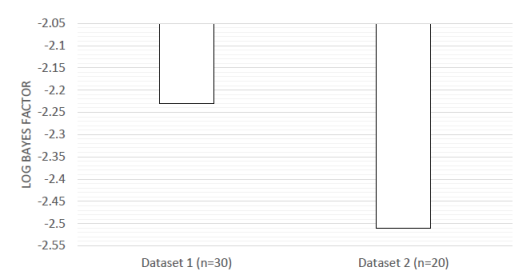
\includegraphics[scale=0.85]{Figures/Comparison_VBA}\caption{Model comparison between old and new versions of the VBA toolbox,
based on two delay fear conditioning datasets. The log Bayes factor
quantifies the difference between negative log likelihood (nLL) of
parameter estimates obtained from model inversion using the old and
new version of VBA. A difference in nLL above 3 indicates significant
differences in model evidence which is not exceeded for either data
set. Analysis and figure contributed by Matthias Staib. \label{fig:VBA}}
\end{figure}


\section{PsPM Version 3.0.1}

\subsection*{Import}

\subsubsection*{New data types were implemented}
\begin{itemize}
\item DATAQ Windaq (no ActiveX needed)
\item European Data Format (EDF)
\end{itemize}

\subsection*{Tools}

'Preprocess respiration traces' replaces 'Convert Respiration to Respiration
Period'. It supports conversions into the following datatypes:
\begin{itemize}
\item Respiration preriod (old funtionality)
\item Respiration amplitude
\item Respiration line length
\item Respiration time stamp
\end{itemize}

\subsection*{First level contrast}

\subsubsection*{Z-score parameter estimates}

The function \texttt{pspm\_con1} now supports z-scoring trial-by-trial
parameter estimates. If selected, all parameter estimates for the
same event type, across all trials, will be z-scored before computing
the contrast. This option is currently only available for non-linear
models.

\subsection*{Review first level model}

Next to the regressors on the x- and y-axes, orthogonality plots newly
display regressor names along the y-axes. 

\section{PsPM Version 3.0.2}

\subsection*{GLM}

Problem with multiple sessions in Design matrix fixed.

\section{PsPM Version 3.1}

\subsection*{General linear modelling (GLM)}

\subsubsection*{New modalities}

For the first time in PsPM, we introduce models for data types other
than SCR:
\begin{itemize}
\item GLM for evoked HPR
\item GLM for fear-conditioned HPR
\item GLM for evoked RA
\item GLM for fear-conditioned RA
\item GLM for evoked RFR
\item GLM for evoked RP
\item GLM for fear-conditioned PS
\end{itemize}

\subsection*{Tools \& Data preprocessing}

Tools are split up into Tools \& Data preprocessing. The content of
each section is listed below. New functions are written in \textcolor{green}{green}.

\subsubsection*{Tools}
\begin{itemize}
\item Display data
\item Rename file
\item Split sessions
\item Artefact removal
\item Downsample data
\item Interpolate missing data
\item \textcolor{green}{Extract segments}
\item \textcolor{green}{Segment mean}
\end{itemize}

\subsubsection*{Data preprocessing}
\begin{itemize}
\item \textcolor{green}{Preprocess heart data}
\item \textcolor{green}{Preprocess respiration data}
\item \textcolor{green}{Prepare illuminance GLM}
\item \textcolor{green}{Find valid fixations}
\item \textcolor{green}{Convert pupil data}
\item \textcolor{green}{Find startle sound onsets}
\end{itemize}

\subsection*{Data preparation}

\subsubsection*{Import}

Support for Philips Scanphyslog files and for bioread-converted AcqKnowledge
files has been added to the import function.

\section{PsPM Version 4.0}

\subsection*{Change from scr\_ to pspm\_}

The prefix scr\_ has been exchanged with pspm\_. This applies to all
functions contained in PsPM.

\subsection*{Updated toolboxes}

Matlabbatch (\url{https://git.code.sf.net/p/matlabbatch/code-git})
and the VBA toolbox (\url{https://github.com/MBB-team/VBA-toolbox})
were updated to the latest available versions (08.11.2016). The updated
VBA version fully supports newer Matlab versions and warning messages
in Matlab 2014 and newer do not appear anymore (during PsPM startup).
In terms of predictive validity, we noted that there was no consistent
benefit of the old or new version of this code (Figure \ref{fig:VBA_compare_3.2}).

\begin{figure}
%\includegraphics[bb = 0 0 200 100, draft, type=eps]{Figures/Comparison_VBA_3.2.png}

\caption{\label{fig:VBA_compare_3.2}Model comparison between old and new versions
of the VBA toolbox, based on one delay fear conditioning dataset (Dataset
2, see earlier comparison). The log Bayes factor quantifies the difference
between negative log likelihood (nLL) of parameter estimates obtained
from model inversion using the old and new version of VBA. A difference
in nLL above 3 indicates significant differences in model evidence
which is not exceeded for the used dataset.}

\end{figure}


\subsection*{Subsessions in DCM models}

Until now, long periods of NaN values (which are just disregarded)
could cause problems for inversion of DCMs. These periods are now
split (according to threshold value) into subsessions. The subsessions
will be evaluated independently, while at the end the results will
be stacked together. Therefore the output-format will not change and
should be compatible with earlier releases.

\subsection*{Import}

\subsubsection*{New import function for Labchart files}

The new import function allows direct import of raw labchart files
without exporting them to a suitable format (as was required to date).
The function is only available on Windows systems.

\subsection*{General linear modeling (GLM)}

\subsubsection*{New modalities}
\begin{itemize}
\item Startle eyeblink for EMG (SEB)
\end{itemize}

\subsection*{Pupil Models}
\begin{itemize}
\item Blink channels were removed. Periods during blinks and saccades are
set to NaN already in the import function. This applies to all channels
of the respective eye. Accordingly, blink validation functionality
was removed in the function pspm\_find\_valid\_fixations. If needed,
blinks and saccades can be imported as custom channels using channel
ids 7-10 (two eyes) or 4-5 (one eye), while blinks and left eye come
first.
\item Importing pupil channels now allows direct specification of a transfer
function to convert arbitrary units to mm. 
\item Importing of eyes which have not been recorded creates channels containing
NaN values, so that the same import batches can be used for groups
of subjects, even if one eye is missing in some of them.
\item Sessions in eyelink files (caused by interruption of recording) will
be concatenated according to the timing variable.
\item In pspm\_find\_valid\_fixations 
\begin{itemize}
\item the use of software aspect ratio was replaced by resolution. This
allows to correctly map the gaze coordinates to the shapes mapped
by the stimulus software.
\item gaze coordinates can be plotted in order to verify the validation
settings.
\item interpolation option was removed and should now be used independently.
\end{itemize}
\end{itemize}

\subsection*{Minor changes \& Bugfixes}
\begin{itemize}
\item Version-Check bug during startup is now fixed.
\item Markerinfos will now according to marker channels be converted to
an event-based format.
\item The data editor (pspm\_data\_editor) now allows to specify an output
file using the command line.
\item pspm\_split\_sessions additionally allows to specify marker ids at
which the file should split.
\item Artefact correction was extended with a further function (Simple SCR
quality correction).
\item Convert pupil data becomes convert data and currently only allows
area to diameter conversion (arbitrary units to mm is integrated in
the import function)
\end{itemize}

\section{PsPM Version 4.0.1}

\subsection*{Bugfixes}
\begin{itemize}
\item Fix not working options in Matlabbatch module 'Preprocess heart data'
\end{itemize}

\section{PsPM Version 4.0.2}

\subsection*{Bugfixes}
\begin{itemize}
\item Fix error when calling 'Convert data' from GUI
\item Fix taking square root if pupil data is recorded in AREA
\end{itemize}

\section{PsPM Version 4.1.0}

\subsection*{New Functions}
\begin{itemize}
\item pspm\_convert\_pixel2unit: Allows to transfer gaze data from pixel
to units. This facilitates the use of pspm\_find\_valid\_fixations
which needs data in unit values.
\item pspm\_compute\_visual\_angle: Computes visual angle from gaze data.
\item pspm\_convert\_visangle2sps: Convert visual angles from Eyelink to
Scanpath speed.
\item pspm\_bf\_spsrf\_box: SPSRF basis function with box car.
\item pspm\_bf\_spsrf\_gamma: SPSRF basis function with gamma function.
\end{itemize}

\subsection*{New Features}
\begin{itemize}
\item pspm\_extract\_segments supports DCM files/structures.
\item GLM for SPS.
\item pspm\_find\_valid\_fixations can now take a bitmap as input.
\item A new way to trim data: Start and end times can be chosen according
to marker name or value.
\item A new function to import SMI iView X EyeTracker files into PsPM.
\item A new function to import ViewPoint EyeTracker files into PsPM.
\end{itemize}

\subsection*{Changes}
\begin{itemize}
\item pspm\_find\_valid\_fixations now computes a circle around the fixation
points when run in fixations mode.
\end{itemize}

\subsection*{Bugfixes}
\begin{itemize}
\item Heart period response function (bf\_hprf) coefficients are fixed according
to the manual
\item pspm\_extract\_segments bugfixes:
\begin{itemize}
\item Fix bugs related to conditions appearing in different sessions.
\end{itemize}
\item pspm\_get\_eyelink now imports markers between two recording sessions
(previously these markers were ``lost'')
\item pspm\_compute\_visual\_angle: Fix bug in range computation.
\item pspm\_ecg2hb: Fix out of bounds error occurring for highly noisy data
with many outliers.
\item pspm\_get\_acq: Fix incorrect linear transformation during ACQ import.
\item pspm\_convert\_unit: Fix incorrect transformations between metric
units and inches.
\item pspm\_resp\_pp: Fix out of bounds error during convolution in cushion
mode.
\item pspm\_pp in 'simple\_qa' mode now uses the default values specified
in pspm\_simple\_qa.
\item Various further bugfixes.
\end{itemize}

\subsection*{Improvements}
\begin{itemize}
\item Blink and saccade channels can be imported with PsPM Eyelink import.
\item GLM structure holds the missing data percentage of each condition
after segment extraction. Further, the decision to exclude conditions
can be made depending on the percentage of missing data.
\item pspm\_extract\_segments now works both with GLM files and already
loaded structures
\item PsPM now checks if SPM is already in MATLAB path. If so, user is asked
to remove it from path before initializing PsPM.
\item pspm\_load1 now returns statistics about conditions with high NaN
ratios.
\item pspm\_extract\_segments now is able to use data stored in GLM/DCM
structures instead of relying the existence of original data files.
\item Multiple new tests to validate the correctness of the functions.
\end{itemize}

\section{PsPM Version 4.1.1}

This is a hotfix release that fixes a few issues with 4.1.0 release.

\subsection*{Changes}
\begin{itemize}
\item pspm\_get\_eyelink now uses the scaling factor from \cite{Hayes:2015a}
for area based arbitrary units to milimeters conversion.
\item pspm\_get\_smi does not perform pixel to milimeters conversion for
pupil data anymore. Pupil values are returned as is in pixel units.
\item pspm\_get\_smi performs pixel to milimeters conversion for gaze data
only if the stimulus resolution in pixels are given as an extra option.
\end{itemize}

\subsection*{Improvements}
\begin{itemize}
\item pspm\_get\_viewpoint is now able to import blink and saccade channels
from sample files as well. In order to enable this feature, event
files must be stored asynchronously in the datafile. See ViewPoint
EyeTracker section in this manual for further information.
\end{itemize}

\section{PsPM Version 4.2.0}

\subsection*{New Functions}
\begin{itemize}
\item A new pupil data preprocessing function
\item A new pupil foreshortening error correction function
\item A new QRS detection algorithm for fMRI environments
\end{itemize}

\subsection*{New Features}
\begin{itemize}
\item Previously, Eyelink import used to discard 50 ms worth of samples
from each side of every blink or saccade period. This behaviour is
preserved; however, sample discard duration can now be set by the
user.
\item Channel processing functions now store extensive historical data in
PsPM files. This data can be printed in table format using the new
utility \texttt{function pspm\_format\_history\_from\_file}
\item Pupil channel is now loaded according to a new precedence order. Refer
to GLM documentation in this manual to learn more.
\end{itemize}

\subsection*{Changes}
\begin{itemize}
\item Eyelink import now returns times and dates in a slightly different
format.
\item Newest version of PsPM is now obtained from the version string in
pspm.sourceforge.net, not from the download link zip file name
\item GLM now uses the \textbf{LAST} channel of a specified modality in
a PsPM file.
\item Nonlinear SCR model (DCM) now does not use the inter-trial interval
duration value (ITI) of the last trial when computing session specific
minimum ITI values. Previously, using these last ITI values would
lead to abnormally small overall min ITI values in some input files,
thereby causing the inference and PCA sections to use less data for
all trials. Now, we prevent this from happening.
\item Eyelink import parameter blink/saccade edge discard factor default
value has been set to 0. This means no extra samples are discarded
around blinks/saccades.
\end{itemize}

\subsection*{Bugfixes}
\begin{itemize}
\item Fix a bug in \texttt{pspm\_extract\_segments} where trial onsets were
not assigned to conditions correctly
\item Fix a bug in Viewpoint import where files in DOS format were being
parsed incorrectly
\item Fix a bug in Eyelink import where blink/saccade periods where misaligned,
causing the function to discard useful data and return noise instead
\end{itemize}

\subsection*{Improvements}
\begin{itemize}
\item New utility functions to make PsPM more compatible across different
operating systems
\item An optimized Eyelink import function that is significantly faster
and more memory efficient than previous versions
\item An optimized SMI event import function that is significantly faster
than the previous version
\item Multiple new tests to validate the correctness of the functions
\item API unification: Now all preprocessing functions use \texttt{channel\_action}
variable to choose what to do with the new channel.
\end{itemize}

\section{PsPM Version 4.2.1}

\subsection*{New Functions}
\begin{itemize}
\item Three new tests (pspm\_hb2hp\_test.m, pspm\_filtfilt\_test.m, pspm\_butter\_test.m)
\end{itemize}

\subsection*{Changes}
\begin{itemize}
\item \texttt{pspm\_display} and \texttt{pspm\_ecg\_editor} do not perform
filtering anymore.
\item Treatment of missing data in DCM is now the same regardless of whether
they are specified as NaN or via model.missing
\item Eyelink import parameter blink/saccade edge discard factor default
value has been set to 0. This means no extra samples are discarded
around blinks/saccades.
\end{itemize}

\subsection*{Bugfixes}
\begin{itemize}
\item Fix a bug in \texttt{pspm\_hb2hp} where the function crashed when
there is no heartbeat left after lower and upper bound filtering of
the heartbeat periods
\item Fix a bug in \texttt{import\_eyelink} which imported more markers
than the number of markers in the actual .asc file
\item Fix a bug in \texttt{pspm\_display} which crashed when trying to plot
ECG signal that contains NaN
\item Fix a bug in \texttt{pspm\_prepdata} which returned only NaN when
input signal contained some NaN values
\item Fix a bug in \texttt{pspm\_version} which crashed when MATLAB was
invoked with \texttt{-nojvm}
\item Fix a bug in \texttt{pspm\_get\_viewpoint} which returned '+,=,+'
lines in the marker list and which crashed when given a viewpoint
data file containing multiple sessions separated with '+,=' type of
markers
\item Fix a bug in \texttt{import\_viewpoint} which created a new session
for every marker containing a '+' somewhere, e.g.: 'CS+'
\item Fix a bug in \texttt{pspm\_get\_events} which was not able to locate
a marker if it occured on the first or last sample in a given datafile
\item Fix a bug in \texttt{pspm\_filtfilt} which crashed when the filter
parameters were of dimension one
\end{itemize}

\section{PsPM Version 4.3.0}

\subsection*{New Features}
\begin{itemize}
\item In \texttt{pspm\_get\_events}, \texttt{import.flank} can be now set
to \texttt{'all'} what would import all markers and data related to
them.
\item \texttt{pspm\_display }allows now to display pupil size units and
the gaze x \& y coordinate units on the y-axis.
\item \texttt{pspm\_extract\_segments }can be used now with raw data and
thus be called easily within another function.
\end{itemize}

\subsection*{Changes}
\begin{itemize}
\item \texttt{pspm\_version} has a new url and thus do not send any warning
about version checks anymore.
\item \texttt{import\_eyelink} do not import markers which are outside the
session end time (\texttt{END} marker).
\item \texttt{import\_eyelink} sends a warning whenever two markers have
the same timestamp.
\item In \texttt{pspm\_get\_eyelink}, \texttt{import.flank} set to \texttt{'all'}.
\item The test of \texttt{pspm\_extract\_segments} was adapted to the new
feature.
\item External functions and libraries were regrouped in one folder called
\texttt{ext.}
\end{itemize}

\subsection*{Bugfixes}
\begin{itemize}
\item Fix a bux in \texttt{pspm\_bf\_lcrf\_gm} and \texttt{pspm\_bf\_ldrf\_gm}
where the offset was wrongly implemented.
\item Fix a bug in \texttt{pspm\_compute\_visual\_angle} where there was
an error in the conversion factor of pixels wrt. to mm.
\end{itemize}

\section{PsPM Version 5.0.0}

\subsection*{New Features}
\begin{itemize}
\item Allow \texttt{pspm\_data\_editor} to load an epoch file.
\item Allow \texttt{pspm\_simple\_qa} to suppress classification of discretisation oscillations as artefacts, to expand artefact windows, and to automatically remove small data islands embedded in artefacts.
\item Allow \texttt{pspm\_simple\_qa} to store the epochs of data that are
filtered out into an output \texttt{.mat} file. The accompanying GUI
editor is available under 'Artefact removal' in the tools section.
\item Allow \texttt{pspm\_convert\_gaze\_distance} to convert from distance
units to degrees or scanpath speed. The accompanying GUI editor is
available under 'Gaze Convert' in the data preprocessing section.
\item Add the possibility to select the flank in the \texttt{Import} module
of the GUI of PsPM.
\item Add the possibility to import DSV (delimiter separated values) as
well as CSV (comma separated values) data files.
\end{itemize}

\subsection*{Changes}
\begin{itemize}
\item Split the data convert functionality in tools into the 'Gaze Convert'
and 'Pupil Size convert' in the data preprocessing section.
\item Factor out blink/saccade edge filtering logic out of \texttt{pspm\_get\_eyelink}
to \texttt{pspm\_blink\_saccade\_filt}.
\item Deprecate edge filtering functionality in \texttt{pspm\_get\_eyelink}.
\item Make \texttt{pspm\_pupil\_correct\_eyelink} use the last gaze channel
when there are multiple gaze x (similarly y) channels in the file.
\item Make \texttt{pspm\_extract\_segments} return NaN percentages and not
ratios.
\end{itemize}

\subsection*{Bugfixes}
\begin{itemize}
\item Scale DCM plot XTick by sample rate.
\item Correct index offset when dealing with the descending flank for continuous
markers.
\item Allow \texttt{pspm\_display} to plot any type of marker channels.
\item Fix \texttt{pspm\_display} behaviour when user tries to load data
with less channels than the data he/she is currently displaying.
\item Fix \texttt{pspm\_split\_sessions} behaviour when the intertrial interval
in the data is random. Add an option \texttt{randomITI} (0 or 1) which
in the latter case it forces the function to evaluate the mean marker
distance using all the markers and not per session. Default value:
0.
\item Remove \texttt{startsWith} and \texttt{endsWith} from all functions
for a better backward compatibility.
\item Fix bug in \texttt{pspm\_trim} which was wrongly defining the starting
trimming point index.
\end{itemize}

\section{PsPM Version 5.1.0}

\subsection*{New Features}
\begin{itemize}
\item PsPM now has an improved GUI with a more eye-friendly colour and typeface.
\item PsPM now has an alternative GUI built by using .mlapp, which shows
consistent a more modern appearance across different platforms.
\end{itemize}

\subsection*{New Functions}
\begin{itemize}
\item pspm\_scr\_pp
\begin{itemize}
\item \texttt{pspm\_scr\_pp} replaces the classic \texttt{pspm\_simple\_qa}.
\item \texttt{pspm\_scr\_pp} now allows users to detect clipping, where
the results can be exported together with the original outcome.
\item \texttt{pspm\_scr\_pp} now allows users to just write artefact epochs
and leave data unchanged.
\end{itemize}
\end{itemize}

\subsection*{Changes}
\begin{itemize}
\item General
\begin{itemize}
\item Dialogs have been rewritten for avoiding endless loops.
\item \textit{Pre-processing} menu has been reconstructed, where \textit{pupil
size convert} and \textit{gaze convert} are now under \textit{pupil
and eye tracking}.
\item PsPM now always generates test data inside the PsPM folder.
\end{itemize}
\item pspm\_interpolate
\begin{itemize}
\item \texttt{pspm\_interpolate} now process data ending with \texttt{NaN}
well without throwing warnings.
\end{itemize}
\item pspm\_find\_sounds
\begin{itemize}
\item \texttt{pspm\_find\_sounds} now throws warning when some data was
excluded due to the strict parameter setting.
\end{itemize}
\item pspm\_split\_sessions
\begin{itemize}
\item \texttt{pspm\_split\_sessions} is now using \texttt{pspm\_trim} for
processing data.
\end{itemize}
\end{itemize}

\subsection*{Bugfixes}
\begin{itemize}
\item pspm\_glm
\begin{itemize}
\item A bug that leads to the failure of selecting left/right eye has been fixed.
\end{itemize}
\item pspm\_load1 and pspm\_dcm
\begin{itemize}
\item A bug that leads to the failure of exporting statistics has been fixed.
\end{itemize}
\item pspm\_resp\_pp
\begin{itemize}
\item A bug that leads to the failure of opening batch for respiration data
processing has been fixed.
\end{itemize}
\item pspm\_scr\_pp
\begin{itemize}
\item A bug that leads to incorrect matrix construction has been fixed.
\end{itemize}
\end{itemize}

\section{PsPM Version 5.1.1}
\subsection*{New Functions}
\begin{itemize}
\item \texttt{pspm\_bf\_data}
\begin{itemize}
\item New function template to allow users creating their own basis functions (bf) from a data vector.
\end{itemize}
\end{itemize}
\subsection*{UI Improvements}
\begin{itemize}
\item PsPM now has an improved GUI for the main screen and \texttt{pspm\_display}.
\item PsPM now uses system specific design for Windows, macOS and Linux.
\item A bug that affects GUI display has been fixed.
\end{itemize}
\subsection*{Bugfixes}
\begin{itemize}
\item \texttt{pspm\_dcm}
\begin{itemize}
\item A bug of channel and data referring that leads to incorrect missing epoch processing has been fixed.
\item \texttt{pspm\_dcm} now handles empty epochs correctly.
\end{itemize}
\item \texttt{pspm\_scr\_pp}
\begin{itemize}
\item A bug that throws warning when using GUI has been fixed.
\end{itemize}
\item \texttt{pspm\_split\_sessions}
\begin{itemize}
\item A bug which leads to GUI crash has been fixed.
\item \texttt{pspm\_split\_sessions} now accepts correct number of data files and missing epoch files in the GUI.
\item \texttt{pspm\_split\_sessions} now processes missing epochs correctly.
\end{itemize}
\end{itemize}

\section{PsPM Version 6.0.0}
This is a major release and may have incompatibility with previous versions.
\subsection*{New features}
\begin{itemize}
\item PsPM now support a develop mode, which allows
  \begin{itemize}
  \item Minimised terminal output
  \item Automagical parameter selection for testing
  \item Always overwrite files.
  \end{itemize}
\item \texttt{pspm\_extract\_segments}
  \begin{itemize}
  \item now allows an optional \textit{z}-score for normalisation.
  \end{itemize}
\item \texttt{pspm\_find\_valid\_fixations}
  \begin{itemize}
  \item now allows processing preprocessed left/right/combined pupil data.
  \end{itemize}
\item \texttt{pspm\_gaze\_pp}
  \begin{itemize}
  \item now allows preprocessing gaze signals.
  \end{itemize}
\item \texttt{pspm\_overwrite}
  \begin{itemize}
  \item now handles the behaviour of overwrite if not defined by the user, and is used where applicable.
  \end{itemize}
\item \texttt{pspm\_time2index}
  \begin{itemize}
  \item now processes adjustable conversion from time to index globally.
  \end{itemize}
\item \texttt{pspm\_update\_chantype}
  \begin{itemize}
  \item now allows generalised behaviour of updating channel types.
  \end{itemize}
\end{itemize}

\subsection*{Bug Fixes}
\begin{itemize}
\item General
  \begin{itemize}
  \item A bug which may lead to failure of pspm path searching has been fixed.
  \item A bug which may display figures in the GUI has been fixed.
  \end{itemize}
\item \texttt{pspm\_bf\_spsrf\_box}
  \begin{itemize}
  \item now uses correct parameter settings.
  \end{itemize}
\item \texttt{pspm\_convert\_ppu2hb}
  \begin{itemize}
  \item terminates if only one pulse is detected.
  \end{itemize}
\item \texttt{pspm\_data\_editor}
  \begin{itemize}
  \item now able to show figures when import a datafile correctly.
  \end{itemize}
\item \texttt{pspm\_dcm}
  \begin{itemize}
  \item now handles missing epochs that start at 0 correctly.
  \item now processes variables properly to make length consistent.
  \end{itemize}
\item \texttt{pspm\_display}
  \begin{itemize}
  \item now displays plots with correct x-axis ranges.
  \end{itemize}
\item \texttt{pspm\_glm}
  \begin{itemize}
  \item now applies correct variable settings.
  \item now produces results correctly when facing many short missing epochs.
  \end{itemize}
\item \texttt{pspm\_interpolate}
  \begin{itemize}
  \item now returns results correctly when applying forced extrapolation.
  \end{itemize}
\item \texttt{pspm\_resp\_pp}
  \begin{itemize}
  \item now allows replace as the channel action properly.
  \end{itemize}
\item \texttt{pspm\_scr\_pp}
  \begin{itemize}
  \item now uses inconsistent variables when delivering missing epochs.
  \item now writes data out properly when epochs are removed.
  \item now properly handles data if the first channel is not \texttt{scr}.
  \end{itemize}
\item \texttt{pspm\_sf}
  \begin{itemize}
  \item now refer to model file correctly.
  \end{itemize}
\item \texttt{pspm\_split\_sessions}
  \begin{itemize}
  \item now processes missing files with an epoch starting at 0~s properly.
  \item now properly catches edge cases.
  \end{itemize}
\item \texttt{ValidSamplesModel}
  \begin{itemize}
  \item now properly throws warnings if histogram counts are zeros.
  \end{itemize}
\end{itemize}

\subsection*{Improvements}
\begin{itemize}
\item General
  \begin{itemize}
  \item now supports loading \texttt{ppg} data.
  \item now displays improved terminal output text.
  \end{itemize}
\item \texttt{pspm\_con1}
  \begin{itemize}
  \item now assesses the statistics in the arguments for throwing warnings when detecting invalid values.
  \end{itemize}
\item \texttt{pspm\_data\_editor}
  \begin{itemize}
  \item now displays the x and y axis label and text according to the input data.
  \item now sorts the epoch list according to the start data point.
  \end{itemize}
\item \texttt{pspm\_get\_marker}
  \begin{itemize}
  \item now detects and update the field \texttt{flank} when applicable.
  \end{itemize}
\item \texttt{pspm\_import}
  \begin{itemize}
  \item now detects and update the field \texttt{flank} when applicable.
  \end{itemize}
\item \texttt{pspm\_load\_data}
  \begin{itemize}
  \item now checks whether the input has an empty channel.
  \item now autofills some variables.
  \end{itemize}
\item \texttt{pspm\_pupil\_pp}
  \begin{itemize}
  \item now calls \texttt{pspm\_load\_data} to load single channels.
  \end{itemize}
\item \texttt{pspm\_rev\_glm}
  \begin{itemize}
  \item now displays normalised data for visualisation purpose only.
  \end{itemize}
\item \texttt{pspm\_write\_channel}
  \begin{itemize}
  \item now checks whether the input has an empty channel.
  \end{itemize}
\end{itemize}

\subsection*{GUI}
\begin{itemize}
\item "Edit defaults" in the GUI is now working properly.
\item GUI typeface is now generalised across the software.
\end{itemize}

\subsection*{For Developers}
\begin{itemize}
\item General
  \begin{itemize}
  \item PsPM now uses \texttt{.editorconfig} to control the indent.
  \item PsPM now uses UTF-8, LF, and MATLAB's soft tab indent as the standard code formatting style.
  \item PsPM now uses test data from the repository PsPM-data.
  \end{itemize}
\item \texttt{pspm\_get\_text\_test}
  \begin{itemize}
  \item A bug, which leaves residual test files after code testing, has been fixed.
  \end{itemize}
\end{itemize}

\section{PsPM Version 6.1.0}
\subsection*{General}
	\begin{itemize}
		\item Minimum version of MATLAB
		\begin{itemize}
			\item The minimum version of MATLAB required for running PsPM is \href{https://uk.mathworks.com/content/dam/mathworks/mathworks-dot-com/support/sysreq/files/SystemRequirements-Release14-ServicePack3_SupportedCompilers.pdf}{MATLAB 7.1 or R14 Service Pack 3}.
		\end{itemize}
		\item Entering PsPM
		\begin{itemize}
			\item Entering PsPM is now hybrid based on the version of MATLAB, namely through AppDesigner or Guide. PsPM will be entered through AppDesigner when supported and through Guide for older versions of MATLAB. To call PsPM, users should still use the command \texttt{pspm} in the Command Window of MATLAB, where the appropriate way of entering PsPM will be recognised automatically.
			\item Users can still use their preferred way to enter PsPM. To enter PsPM through AppDesigner, please type \texttt{pspm\_appdesigner}. To enter PsPM through Guide, which is the classic entrance, please type \texttt{pspm\_guide}.
			\item The AppDesigner version of PsPM UI is newly introduced by MATLAB and the encouraged way for launching PsPM, and it has no functionality difference than the Guide version of PsPM UI.
			\item Both AppDesigner and Guide are designed and tested for Windows, macOS (either Intel or Apple Silicon) and Linux. Issues of opening PsPM through either of the two UI systems are encouraged to be reported to PsPM developing group at GitHub.
		\end{itemize}
		\item Introducing \texttt{pspm\_options}
		\begin{itemize}
			\item A new function \texttt{pspm\_options} is introduced to PsPM for controlling the default and acceptable values of the struct \texttt{options} used by most PsPM functions. The default values of the fields in the struct \texttt{options} for various functions can be directly checked by searching in \texttt{pspm\_options}.
			\item The default values in \texttt{pspm\_options} have been checked and tested for PsPM. If preferred values are different from defaults, users can specify them when calling the corresponding PsPM functions, and the corresponding functions and \texttt{pspm\_options} will always respect the users' specification with the highest priority. However, the user's specification needs to satisfy the condition set in \texttt{pspm\_options}, and invalid values may be reported as errors.
		\end{itemize}
		\item UI Improvements
		\begin{itemize}
			\item The UI for the following features has been improved and tested
			\begin{itemize}
				\item Launchpad (AppDesigner)
				\item Launchpad (Guide)
				\item Batch editor
				\item Display data
				\item Contrast manager
			\end{itemize}
		\end{itemize}
		\item Help text
		\begin{itemize}
			\item The help text has been updated for all PsPM functions. Help text can be checked by right clicking the functions.
		\end{itemize}
	\end{itemize}
\subsection*{Bug Fixes}
	\begin{itemize}
		\item UI
		\begin{itemize}
			\item A bug that used to make PsPM crash when \textit{Pupil size convert} and \textit{Gaze convert} in \textit{Data Preprocessing} were selected has been fixed.
			\item A bug that leads to error when PsPM is started offline has been fixed.
			\item A bug that leads to incorrect x labels in \texttt{pspm\_rev\_dcm} has been fixed.
		\end{itemize}
		\item \texttt{pspm\_convert\_...}
		\begin{itemize}
			\item A bug that leads PsPM to crash, which is caused by outdated UI calling for \texttt{pspm\_convert\_...} functions, has been fixed.
		\end{itemize}
		\item \texttt{pspm\_get\_eyelink}
		\begin{itemize}
			\item A bug that causes issues when importing eye link data that is scanned at both left and right sides has been fixed.
		\end{itemize}
		\item \texttt{pspm\_glm}
		\begin{itemize}
			\item A bug that incorrectly identifies the NaNs in the input data has been fixed.
		\end{itemize}
		\item \texttt{pspm\_sf}
		\begin{itemize}
			\item A bug that has lead to incorrect input datafile assigning has been fixed.
			\item A bug that leads PsPM crash when \texttt{pspm\_sf} is analysing data with missing epochs has been fixed.
			\item A bug that leads to error when \texttt{pspm\_sf} analyses data where \texttt{time unit} is defined as \texttt{marker} has been fixed.
		\end{itemize}
		\item \texttt{pspm\_split\_sessions}
		\begin{itemize}
			\item \texttt{pspm\_split\_sessions} now considers \texttt{marker\_chan\_num} when calling \texttt{pspm\_trim}.
		\end{itemize}
	\end{itemize}
	
\subsection*{Improvements}
    \begin{itemize}
    	\item \texttt{channel}
    	\begin{itemize}
    		\item We have generalised \texttt{channel} related variables throughout PsPM, which are given as 
    		\begin{itemize}
    			\item \texttt{chan/channel} to \texttt{channel}
    			\item \texttt{chans/channels} to \texttt{channels}
    			\item \texttt{channel\_units/channels\_units/chan\_units/chans\_units} to \texttt{channel\_units}
    			\item \texttt{chan\_combine} to \texttt{channel\_combine}
    			\item \texttt{chan\_action} to \texttt{channel\_action}
    			\item \texttt{channels\_header} to \texttt{channel\_header}
    			\item \texttt{chantype} to \texttt{channeltype}
    		\end{itemize}
			\end{itemize}
    	\item \texttt{import\_eyelink}
    	\begin{itemize}
    		\item Improved \texttt{import\_eyelink} for adding some support for importing eyelink data converted by higher version of .EDF files.
    	\end{itemize}
    	\item \texttt{pspm\_con2}
    	\begin{itemize}
    		\item \texttt{pspm\_con2} is now using \texttt{pspm\_overwrite}.
    	\end{itemize}
    	\item \texttt{pspm\_dcm} and \texttt{pspm\_dcm\_inv}
    	\begin{itemize}
    		\item \texttt{.flexevents} and \texttt{.fixevents} are now fields of \texttt{model} instead of \texttt{options}.
    		\item \texttt{pspm\_dcm} now uses \texttt{pspm\_get\_timing} to handle missing epochs.
    		\item Improved missing epoch support
    		\begin{itemize}
    			\item The field \texttt{.missing} is now allocated from \texttt{options} to \texttt{model}.
    			\item \texttt{.missing\_data} is used to load missing epoch data that was loaded from dcm, as an optional field.
    		\end{itemize}
    		\item The index is changed so that the first event will not be excluded when at time 0 in session.
    	\end{itemize}
    	\item \texttt{pspm\_extract\_segments}
    	\begin{itemize}
    		\item The first channel is always referred by \texttt{marker\_chan} as default.
    	\end{itemize}
    	\item \texttt{pspm\_glm}
    	\begin{itemize}
    		\item The fallback for \texttt{options.exclude\_missing} has been set for \texttt{pspm\_glm}, which is not to exclude any missing epochs.
    		\item A bug that leads to incorrect missing epoch checking has been fixed.
    		\item Help text was updated.
    		\item \texttt{marker\_chan\_num} now refers to the first marker channel as default.
    		\item \texttt{pspm\_glm} now uses \texttt{pspm\_get\_timing} to handle missing epochs.
    	\end{itemize}
    	\item \texttt{pspm\_interp1}
    	\begin{itemize}
    		\item \texttt{pspm\_interp1} now considers the data where no valid values are detected and interpolation is not possible, and warnings will be reported in this case.
    	\end{itemize}
    	\item \texttt{pspm\_merge}
    	\begin{itemize}
    		\item The default value is set to be [1,2], meaning the first channel will be merged as the default option.
    	\end{itemize}
    	\item \texttt{pspm\_prepdata}
    	\begin{itemize}
    		\item \texttt{pspm\_prepdata} now uses interpolation to handle data with \texttt{NaN}.
    		\begin{itemize}
    		\item Data that begins and/or ends with \texttt{NaN} will be filled with the first/last non-\texttt{NaN} values in those positions.
    		\end{itemize}
    	\end{itemize}
    	\item \texttt{pspm\_sf}
    	\begin{itemize}
    		\item \texttt{pspm\_sf} now supports missing epochs.
    		\begin{itemize}
    			\item Now allow input with \texttt{NaN} that indicates missing epochs. 
    			\item Missing epochs can be specified with options.missing or the automatic \texttt{NaN} detection. 
    			\item Missing epochs will be verified with \texttt{options.missingthresh}. 
    			\item When the missing epochs are longer than 2s, the result out will be converted to \texttt{[]}.
    			\item The UI of SF analysis now allows using missing epochs from files or not to define any missing epochs.
    		\end{itemize}
    		\item \texttt{pspm\_sf} now uses \texttt{pspm\_get\_timing} to handle missing epochs.
    		\item \texttt{marker\_chan\_num} now refers to the first marker channel as default.
    	\end{itemize}
    	\item \texttt{pspm\_sf\_dcm}
    	\begin{itemize}
    		\item \texttt{pspm\_sf\_dcm} now uses \texttt{pspm\_interp1} for interpolating data.
    	\end{itemize}
    	\item \texttt{pspm\_text}
    	\begin{itemize}
    		\item The Matlab file that stores the information of help text \texttt{pspm\_text.mat} will be stored inside the source folder of PsPM and will be deleted when PsPM is quit.
    	\end{itemize}
    	\item \texttt{pspm\_trim}
    	\begin{itemize}
    		\item \texttt{marker\_chan\_num} now refers to the first marker channel as default.
    	\end{itemize}
    \end{itemize}
    
\subsection*{Minor Adjustments}
    \begin{itemize}
    	\item \texttt{pspm\_sf}, \texttt{pspm\_glm} and \texttt{pspm\_dcm}.
    	\begin{itemize}
    		\item The option \texttt{marker\_chan\_num\_event} is removed.
    		\item In default, the first marker channel / event channel is always selected and no users' customisation is allowed.
    		\item The last data channel / wave channel is always selected.
    	\end{itemize}
    \end{itemize}
\subsection*{Reference document}
    \begin{itemize}
    	\item New document \textit{PsPM Reference} for checking the default values and restrictions of \texttt{options} fields.
    \end{itemize}

\section{PsPM Version 6.1.1}

\subsection*{New features}
\begin{itemize}
\item \texttt{pspm\_bf\_psrf\_2\_fc}
\begin{itemize}
\item \texttt{pspm\_bf\_psrf\_2\_fc} now allows to set the time delay between
CS and US.
\item Previously, \texttt{pspm\_bf\_psrf\_2\_fc} used to set a basis function
for the CS and for the US response with a time delay of 3.5 s as standard.
\end{itemize}
\item \texttt{pspm\_dcm}
\begin{itemize}
\item Missing data epochs from file and data can be combined.
\end{itemize}
\item \texttt{pspm\_glm}
\begin{itemize}
\item \texttt{pspm\_glm} now allows a two-element vector and construct the
dictionary accordingly.
\item Previously \texttt{pspm\_glm} only allows scalar values in model.window.
\end{itemize}
\end{itemize}

\subsection*{New functions}
\begin{itemize}
\item \texttt{pspm\_check\_model}
\begin{itemize}
\item \texttt{pspm\_check\_model} checks the fiels of models.
\end{itemize}
\item \texttt{pspm\_combine\_markerchannels}
\begin{itemize}
\item \texttt{pspm\_combine\_markerchannels} allows users to use the GLM
option \textquotedbl markervalues\textquotedbl{} to create onsets
definition from channels distributed across multiple channels.
\end{itemize}
\item \texttt{pspm\_tam}
\begin{itemize}
\item \texttt{TAM} stands for Trial Average Model. \texttt{pspm\_tam} allows
to fit models on trial-averaged data. 
\end{itemize}
\end{itemize}

\subsection*{Adjustments}
\begin{itemize}
\item \texttt{pspm\_pupil\_pp}
\begin{itemize}
\item Now \texttt{pspm\_pupil\_pp} creates channels of type \texttt{pupil}
rather than \texttt{pupil\_pp}.
\end{itemize}
\item \texttt{pspm\_split\_sessions}
\begin{itemize}
\item \texttt{pspm\_split\_sessions} no longer drops markers at beginning
or end of file. 
\end{itemize}
\end{itemize}

\subsection*{Bug fixes}
\begin{itemize}
\item \texttt{pspm\_con}
\begin{itemize}
\item A bug caused by the new varargout logic of \texttt{pspm\_load1} has
been fixed.
\end{itemize}
\item \texttt{pspm\_dcm}
\begin{itemize}
\item A bug that leads dropping sub-threshold missing data periods has been
fixed.
\end{itemize}
\item \texttt{pspm\_get\_spike}
\begin{itemize}
\item A minor bug caused by a non-existing variable has been fxied.
\end{itemize}
\item \texttt{pspm\_scr\_pp}
\begin{itemize}
\item A bug that could change the original file if it saves epochs to \texttt{missing\_epoch.mat}
has been fixed. 
\end{itemize}
\end{itemize}

\subsection*{Improvements}
\begin{itemize}
\item \texttt{pspm\_extract\_segments}
\begin{itemize}
\item Now \texttt{pspm\_extract\_segments} process the data after excluding
the missing data information that is provided in the model structure.
\end{itemize}
\item \texttt{pspm\_dcm}
\begin{itemize}
\item Processed data are now initialised as data matrix with \texttt{NaN}
before inserting data of variable size.
\end{itemize}
\item \texttt{pspm\_glm}
\begin{itemize}
\item A warning has been added if any duration in onset definition is above
\texttt{0} and modality is not \texttt{sps}.
\end{itemize}
\item \texttt{pspm\_overwrite}
\begin{itemize}
\item The logic of overwriting files in PsPM has been updated.
\item Specifically, the overwriting operation is applicable only if there
has been a file with the proposed name of the outputfile.
\item A warning will be provided if the user chooses not to overwrite the
file, since the output of PsPM will not be saved. 
\end{itemize}
\item \texttt{pspm\_split\_sessions}
\begin{itemize}
\item A misleading warning provided by \texttt{pspm\_split\_sessions} when
it processes a missing epoch file has been fixed.
\item The help text of \texttt{split\_sessions} in the GUI has been updated.
\end{itemize}
\end{itemize}

\subsection*{UI improvements}
\begin{itemize}
\item PsPM's UI in Linux environment has been improved.
\end{itemize}


\section{PsPM Version 6.1.2 }
\subsection*{Bug fixes}
\begin{itemize}
\item GUI
\begin{itemize}
\item A bug that made channel actions in EMG pre-processing unrecognised has been fixed.
\item A bug, which sometimes made DCM not run from the GUI, has been fixed.
\end{itemize}
\item \texttt{pspm\_convert\_hb2hp}
\begin{itemize}
\item A bug, which incorrectly selected heart rate channels, has been
fixed.
\end{itemize}
\item \texttt{pspm\_dcm}
\begin{itemize}
\item A bug, which could lead to a wrong sample rate being used if more than one SCR channel existed in the file, has been fixed.
\end{itemize}
\item \texttt{pspm\_glm}
\begin{itemize}
\item A bug, which leads to markers being taken from the first marker
channel but markervalues from the last, has been fixed.
\end{itemize}
\end{itemize}

\bibliographystyle{pnas2009}
\bibliography{PsPM}

\end{document}
